\RequirePackage{xcolor}
\documentclass[journal,twoside,web]{ieeecolor}
\usepackage{jsen}
\usepackage{cite}
\usepackage{amsmath,amssymb,amsfonts}
\usepackage{graphicx}
\usepackage{textcomp}
\usepackage{wrapfig}
\usepackage{amssymb}
\usepackage{xcolor}
\usepackage{algorithmic}
\usepackage{array}
\usepackage{stfloats}
\usepackage{url}
\usepackage{epstopdf}
\usepackage{subfigure}
\usepackage{epsfig}
\usepackage{tikz}
\usepackage{dcolumn}
\usepackage{bm}
\usepackage{color}
\usepackage{accents}
\usepackage{braket}
\usepackage{mathtools}
\usepackage{tabularx}
\usepackage{nicefrac}
\usepackage{booktabs}
\usepackage{array}
\usepackage{multirow}
\usepackage[geometry]{ifsym}
\usepackage[T1]{fontenc}
\usepackage{cleveref}
%Definition of donde se dejan las imagenes
\graphicspath{ {./figures/} }
%Definition colour comments
\definecolor{javcolor}{rgb}{1.00, 0.0, 0.00}
\newcommand{\javnote}[1]{\textcolor{javcolor}{#1}}
%Definition colour
\definecolor{inicolor}{rgb}{0.0, 0.0, 1.00}
\newcommand{\ininote}[1]{\textcolor{inicolor}{#1}}
\definecolor{inacolor}{rgb}{0.0, 1.0, 1.00}
\newcommand{\inanote}[1]{\textcolor{inacolor}{#1}}
\newcommand*{\tikzbullet}[2]{%
  \setbox0=\hbox{\strut}%
  \begin{tikzpicture}
    \useasboundingbox (-.2em,0) rectangle (.2em,\ht0);
    \filldraw[draw=#1,fill=#2] (0,0.3\ht0) circle[radius=.2em];
  \end{tikzpicture}%
}
% Comando personalizado para cuadrados
\newcommand{\squarecolor}[1][black]{%
	\tikz\draw[fill=#1] (0,0) rectangle (0.2,0.2);%
}
\newcolumntype{N}{>{\centering\arraybackslash}m{.5in}}
\newcolumntype{M}{>{\centering\arraybackslash}m{0.7in}}
\newcolumntype{G}{>{\centering\arraybackslash}m{2in}}
\newcommand{\markerone}{\raisebox{0.5pt}{\tikz{\node[draw,scale=0.4,circle,fill=black!20!blue](){};}}}
\newcommand{\markertwo}{\raisebox{0pt}{\tikz{\node[draw,scale=0.3,regular polygon, regular polygon sides=3,fill=black!45!green,rotate=180](){};}}}
\newcommand{\markerthree}{\raisebox{0.5pt}{\tikz{\node[draw,scale=0.3,regular polygon, regular polygon sides=3,fill=black!10!red,rotate=0](){};}}}
\newcommand{\markerfour}{\raisebox{0.5pt}{\tikz{\node[draw,scale=0.4,regular polygon, regular polygon sides=4,fill=none](){};}}}
\newcommand{\markerfive}{\raisebox{0pt}{\tikz{\node[draw,scale=0.4,diamond,fill=black!10!gray](){};}}}
\newcommand{\markersix}{\raisebox{0.6pt}{\tikz{\node[draw,scale=0.3,circle,fill=black!100!](){};}}}
\def\BibTeX{{\rm B\kern-.05em{\sc i\kern-.025em b}\kern-.08em
    T\kern-.1667em\lower.7ex\hbox{E}\kern-.125emX}}
\markboth{\journalname, VOL. XX, NO. XX, XXXX 2022}
{Author \MakeLowercase{\textit{et al.}}: Preparation of Papers for IEEE TRANSACTIONS and JOURNALS (February 2017)}
\definecolor{abstractbg}{rgb}{0.89804,0.94510,0.83137}
\setlength{\fboxrule}{0pt}
\setlength{\fboxsep}{0pt}
\begin{document}
\title{Boosting the Performance of Planar CSRR Sensors in Biomedical Applications Through Machine Learning}
\author{Javier Alonso-Valdesueiro, Luis Fernández, Agustín Gutiérrez-Gálvez, and Santiago Marco-Colás
\thanks{J. Alonso-Valdesueiro is with University of Barcelona, Carrer Martí i Franquès,1. 08028, Barcelona, Spain (e-mail: javier.alonsov@ub.edu). }
\thanks{L. Fernández, is with University of Barcelona, Carrer Martí i Franquès,1. 08028, Barcelona, Spain (e-mail: lfernandez@ub.edu).}
\thanks{A. Gutiérrez-Gálvez, is with University of Barcelona, Carrer Martí i Franquès,1. 08028, Barcelona, Spain (e-mail: agutierrez@ub.edu).}
\thanks{S. Marco-Colás, is with University of Barcelona, Carrer Martí i Franquès,1. 08028, Barcelona, Spain (e-mail: santiago.marco@ub.edu) and the Institute for Biomedical Engineering of Catalonia (IBEC), Carrer Baldiri i Reixac, 4, Torre R. 08028, Barcelona, Spain (email: smarco@ibecbarcelona.eu).}}

\IEEEtitleabstractindextext{%
\fcolorbox{abstractbg}{abstractbg}{%
\begin{minipage}{\textwidth}%
\begin{wrapfigure}[18]{r}{3in}%
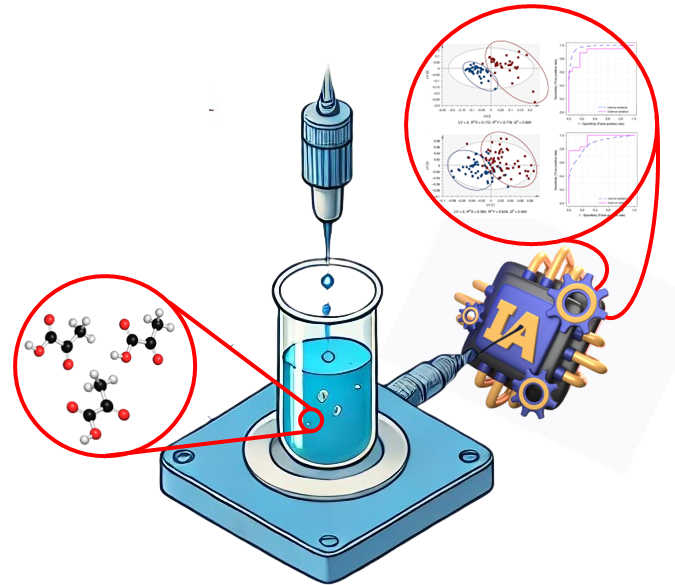
\includegraphics[width=2.5in]{figures/fig0.png}%
\end{wrapfigure}%
\begin{abstract}
Complementary Split Ring Resonators have been developed as planar sensors over the last decade. Changes in the electromagnetic properties ($\epsilon$ and $\delta$) on their surfaces produce responses in their Scattering Parameters (S-Parameters), which can be measured with a Vector Network Analyzer (VNA). Despite their success as sensors, their applicability has been constrained to laboratory experiments, where highly accurate VNAs are used, environmental conditions are meticulously controlled, and the Sample Under Test (SUT) is carefully accommodated to the peculiarities of the sensors. Additionally, their performance has been evaluated in terms of linearity, sensitivity, and accuracy, without considering the practical applicability of this technology. In this contribution, a new approach is proposed. Considering the potential application of this technology in biomedical research, the equipment used for the measurement of the S-Parameters (the VNA) is an inexpensive, portable device, the SUT is placed inside a test vial commonly used in biomedical research, and the environmental conditions during sampling are not controlled. From this starting point, measurements of benchmark SUT samples (ethanol mixed with deionized water in different concentrations) have been performed randomly, and a Principal Component Analysis of the acquired database has been carried out for data visualization. Subsequently, a Partial Least Squares Regressor has been trained and evaluated in terms of Root Mean Square Error in the test phase. The trained model is capable of quantifying bi-component substances such as ethanol and deionized water with an RMSE of approximately $3.7\%$ and a Limit of Agreement of approximately $15\%$ within a $95\%$ Confidence Interval.           
\end{abstract} 

\begin{IEEEkeywords}
CSRR Sensors, Machine Learning, RF Biomedical, Resonators.
\end{IEEEkeywords}
\end{minipage}}}
\maketitle
\section{Introduction}
\label{sec:intro}
\IEEEPARstart{C}{omplementary} Split Ring Resonators (CSRR) were introduced as metasurfaces and metamaterials~\cite{falcone2004, Baena2005}. They were designed to act as microwave stopband and notch filters, transmission lines, and antennas~\cite{GGarcia2005, Bonache2006, Mandal2006, Gil2007, Velez2008, Zhang2009}. However, due to their sharp behavior as filters and the influence of surface surroundings on their performance~\cite{Grzegorczyk2005, Stevanovic2006, Bonache2006}, they started to be used as sensors a few years after their first appearance~\cite{Boybay2012}. Since then, several applications have focused on measuring the complex permittivity of different materials~\cite{Song2013, Lee2014, Lee2014_2, Ansari2015, Standaert2017, Su2019}.

In the last five to seven years, CSRR sensors have been increasingly used in biomedical applications to measure the dielectric properties of different solutions and concentrations of solutes in solvents~\cite{Velez2018, Omer2021, Zhang2019}. Some applications have attracted particular attention during this period (such as glucose concentration quantification in water~\cite{Omer2021, Martinic2025}), but most studies have focused on developing CSRR sensors for microfluidic devices applied to various fields~\cite{Patel2022, Jiang2023, Liu2024, Zhang2024}.

The use of statistical learning tools (or Machine Learning algorithms) to enhance the performance of CSRR-based devices has also been explored over the past five years~\cite{Prakash2022, Harrison2020, Kazemi2022, Abdolrazzaghi2023}. These algorithms have been employed as fitting tools to generalize the dependence of certain features of the CSRR S-parameters (such as frequency resonances, magnitude values, and phase distortion)  on the dielectric properties of the samples~\cite{Martinic2025}. Moreover, in recent years, their use has expanded to include Multivariate Analysis (MVA) for correlating solute concentrations in water~\cite{Trovarello2024}.

However, the full potential of ML algorithms applied to data from CSRR sensors has not yet been fully explored. These algorithms can generate quantification models that minimize the variability (or noise) present in sensor readings~\cite{Mitchell1997, Wold1987, Wold2001, Nirmal2021}. ML models are capable of identifying common features in the data that allow correlation with specific characteristics of the sample under test (SUT)~\cite{Loutchanwot2022}. In this sense, ML algorithms can improve the performance of noisy, low-selectivity systems and reduce uncertainties introduced during sampling.

In this contribution, the applicability of ML algorithms—specifically, Principal Component Analysis (PCA) and Partial Least Squares Regression (PLSR)—is investigated as a means to enhance the performance of a CSRR-based system. The proposed benchtop device is designed to be portable and low-cost, which introduces uncertainties due to the CSRR sensor, the Vector Network Analyzer (VNA) used to measure the S-parameters, and the sampling methodology. 

The text is organized as follows: In Section~\ref{sec:csrrbenchTop}, the measurement system is briefly described, including the main characteristics of the CSRR sensor and the low-cost VNA used to measure the S$_{21}$ parameter. Section~\ref{sec:mlCSRRs} presents the sample preparation process and characterization using the CSRR measurement system. Additionally, the proposed workflow for statistical learning analysis is introduced and described in its two main approaches: PCA and PLSR. In Section~\ref{sec:csrrPerformance}, the performance of the CSRR system in quantifying the concentration of components in a binary solution is analyzed and discussed. Finally, Section~\ref{sec:conclusion} summarizes the key findings of this study and discusses their potential applications in various fields.        

\section{CSRR benchtop System}\label{sec:csrrbenchTop}
\subsection{System Block Diagram}\label{ssec:sysBlockD}

\begin{figure}[!t]
	\centering
	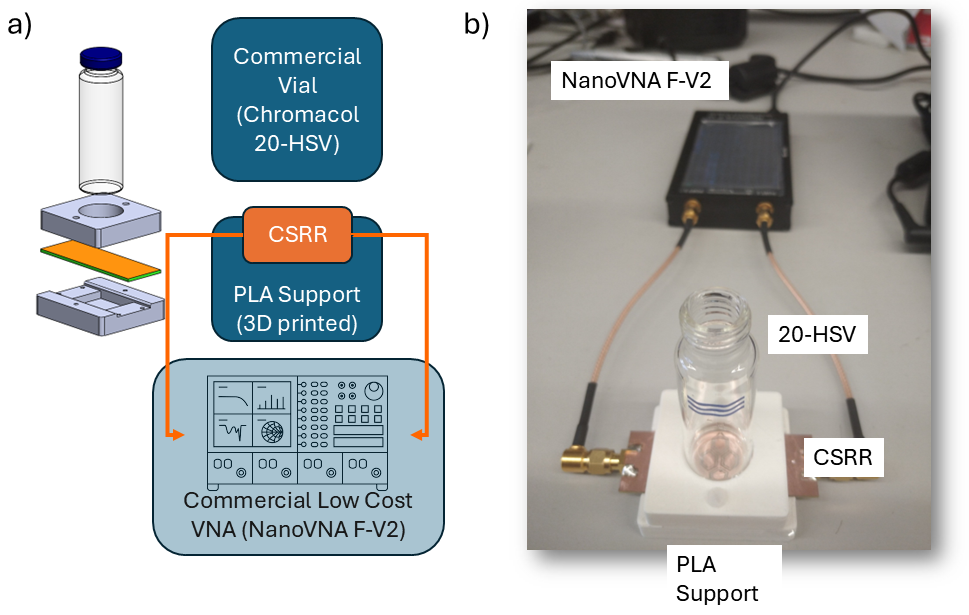
\includegraphics [trim = 0mm 0mm 0mm 0mm, clip, width=1\columnwidth]{figures/fig1.png}
	\caption{Proposed bench-top CSRR system. a) The commercial vial (Chromacol 20-HSV) containing the SUT is placed on the CSRR using a PLA 3D printed support. The CSRR is connected to the low cost VNA (NanoVNA F-V2) by two sma cables. The NanoVNA can be operated via graphical interface running in the device or serial commands coming from an application running in a common laptop. b) Real setup with a vial on top of the CSRR.}
	\label{fig:senBlockD}
	\vspace{-0.3cm}
\end{figure}

Figure~\ref{fig:senBlockD}~(a) shows the block diagram of the CSRR based system. The importance of describing the measurement system comes from the fact that, as it has been discussed in section~\ref{sec:intro}, in the literature, measurement systems are optimized for extracting the best performance of the sensors. 

In this contribution, the CSRR system is thought to be used as a bench-top tool in a biomedical laboratory. Therefore, the Sample Under Test (SUT) is presented to the sensor in a commercial vial (Chromacol 20-HSV). Its position on top of the sensor is ensured by a PLA holder 3D-printed. This holder keeps the CSRR still during measurements and ensures that the commercial vial is placed always centred with respect to the resonant structure of the CSRR sensor. 

The measurement device in a bench-top equipment, must be small, portable, and, if possible, affordable for being placed at any laboratory. In this case, the equipment must measure the S-parameters, in particular, the S$_{21}$. In some contributions, specific electronics were developed for the purpose of measuring this parameter~\cite{Omer2020, Omer2021}. In many other contributions, commercial, high quality and expensive devices are used~\cite{Patel2022, Jiang2023, Liu2024}. However, in this study, a commercial low-cost VNA was chosen as measurement platform (NanoVNA F-V2). This choice is based on the device  affordability, performance in the 1 to 3~GHz band, and operability with an external laptop via serial commands.

Finally, the VNA is connected to a controlling GUI developed in python and running in a commercial lap-top. The GUI allows to acquire data, record it in a comprehensive structure for generating a useful database and run in a continuous measurement mode. Also, it includes a quantification module to accommodate the resulting ML models after training and make predictions of concentration from measurements de S-parameter.   
\subsection{CSRR Sensor}
\label{ssec:csrrSensor}

\begin{figure}[!t]
	\centering
	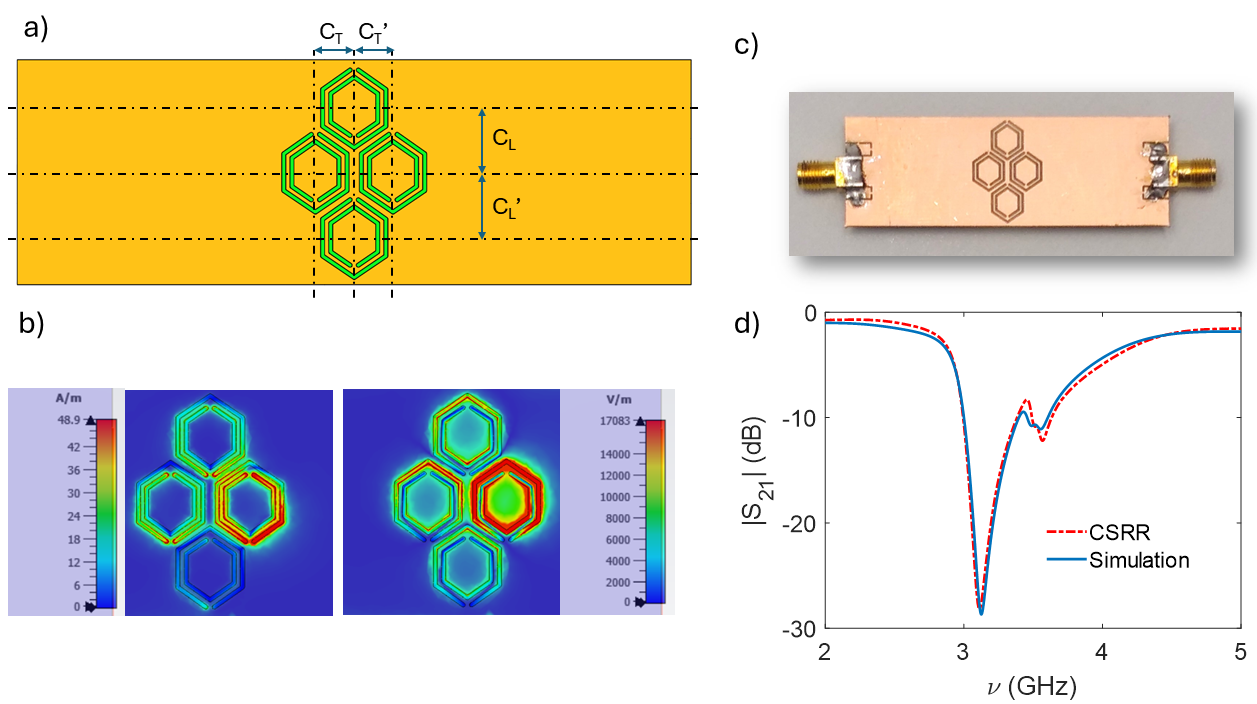
\includegraphics [trim = 0mm 0mm 0mm 0mm, clip, width=1\columnwidth]{figures/fig2.png}
	\caption{Modified CSRR. a) Structure of the measured CSRR with certain modifications. The honeycombs are not placed equidistantly to the centrer of the PCB ($22\times66$~mm). The longitudinal honeycombs are placed at C$_{L}=6.3$ and C$_{L}'=6.4$~mm away from the centrer of the PCB and the transverse honeycombs are placed C$_{T}=3.7$ and C$_{T}'=3.8$~mm away from the centrer of the PCB. b) Simulated electric ($\vec{E}$~\nicefrac{V}{m}) and magnetic field ($\vec{H}$~\nicefrac{A}{m}) in the surface of the multiple honeycomb structure. c) CSRR mounted with sma connectors. d) S$_{21}$ comparison between simulations and measurements (Keisight E5071C-240).}
	\label{fig:csrr}
	\vspace{-0.3cm}
\end{figure}

Figure~\ref{fig:csrr}~(a) shows the structure of the CSRR used in this contribution and the PCB manufactured by Eurocircuits NV. Its structure is based on the honeycomb CSRR presented in~\cite{Omer2020}. However, in order to present some extra features in the S$_{21}$ parameter, some of its dimensions were modified. In particular, the symmetry of the vertical and horizontal combination of honeycombs was modified by 100~$\mu$m. This modification provided to CSRR with an extra feature ($\sim3.5$~GHz) close to the main resonance ($3.2$~GHz). This extra resonance comes from the fact that, the resonator presented here shows asymmetries in the horizontal and vertical plane. Therefore, it is expected to observe some directionality when measuring the S$_{21}$ with a SUT placed on top of the resonator.

The coupling transmission line and the dimensions of each honeycomb are as defined in~\cite{Omer2020}, so the CSRR does not introduce further uncertainty in the measurement.

\section{Machine Learning Algorithms for CSSR sensors}
\label{sec:mlCSRRs}

\subsection{Measurements}
\label{ssec:mlMeasurement}
\subsubsection{System Characterization}
\label{sssec:sysCharac}
In order to characterize the response of the CSRR system to samples with different concentrations of Ethanol diluted in clean water when poured in a commercial vial (Chromacol 20-HSV), a measurement campaign was conducted. The sampling method consisted in measuring vials randomly chosen between a set of $100$ vials for each of the ethanol concentrations considered ($0$ to $96\%$ concentration diluted in clean water). Each vial was taken manually from a containing box, placed on top of the CSRR by the PLA holder and filled up with $1.2$~mL of the corresponding solution.  

This method produced $100$ repetitions of the S$_{21}$ parameter for each concentration, each measured with a different vial. Figure~\ref{fig:avgData} shows the results for each concentration when averaging the $100$ measurements of the $20\dot{\log\left(|S_{21}|\right)}$ and their standard deviation in $\%$.  

\begin{figure}[!t]
	\centering
	\subfigure{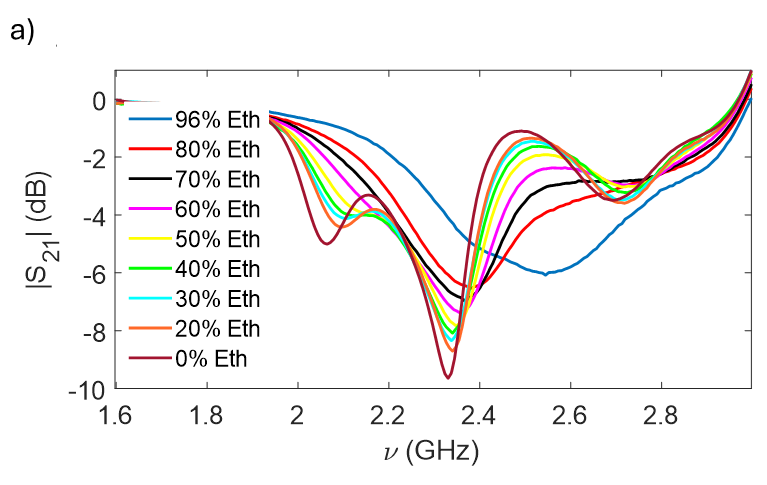
\includegraphics [trim = 0mm 0mm 0mm 0mm, clip, width=1\columnwidth]{figures/fig3_a.png}}
	\subfigure{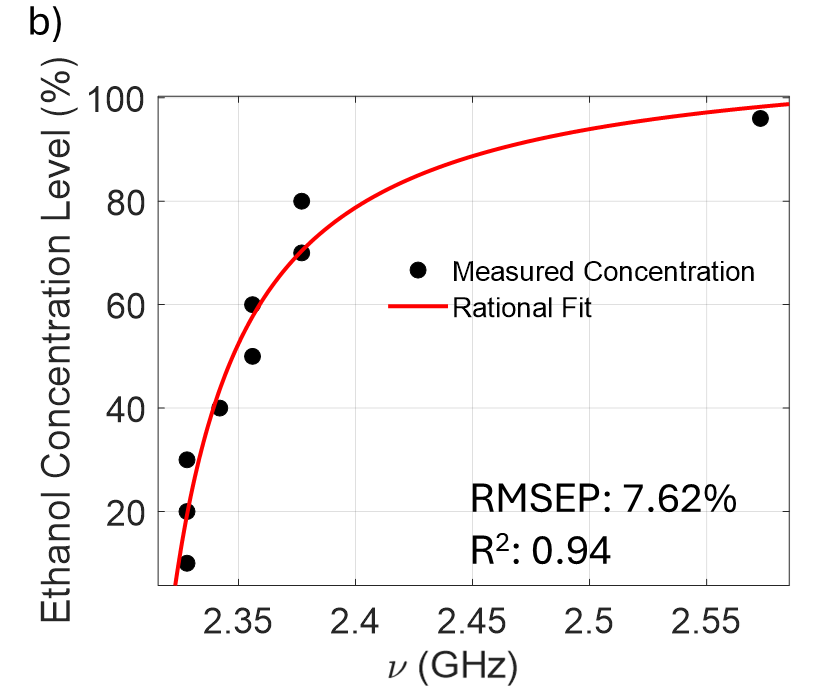
\includegraphics [trim = 0mm 0mm 0mm 0mm, clip, width=1\columnwidth]{figures/fig3_b.png}}
	%\hfill
	\caption{Characterization of the CSRR system when measuring concentrations of ethanol diluted in clean water and poured in commercial vials. a) Averaged $20\dot{\log\left(|S_{21}|\right)}$ response of the CSRR over $100$ repetitions, each from a different vial. b) Standard deviation, in dB, for the repetitions performed with each of the concentrations ($0$, $20$, $30$, $40$, $50$, $60$, $70$, $80$, and $96$~$\%$ of ethanol en clean water.)}
	\label{fig:avgData}
\end{figure}

Figure~\ref{fig:avgData}~(a) shows how the ethanol dumps the S$_{21}$ parameter of the CSRR promoting an increase of the resonance frequency. Also, the evolution of the shape of the S$_{21}$ parameter with the concentration implies a non-linear response of the system with ethanol concentration compared with other studies presented in the literature~\cite{Abdolrazzaghi2023}. Evaluating the frequency displacement of the most prominent resonance in Figure~\ref{avgData}~(a), an exponential fitting of the deepest resonance results in the following expression:

\begin{equation}
	\label{eq:frequFitt}
	 C_{\%}(\nu) = ae^{b\nu}+ce^{d\nu} 
\end{equation} 

when the frequency,$\nu$ is in GHz and a$=80.8512$~$\%$, b$=0.0669$, c$=-7.3475$~$\%$, and d$=-3.8271$. This coefficients are obtained by normalizing $\nu$ with $\mu=2.371$~GHz and $\sigma=66.16$~MHz applying Non Linear Least Squares. The R$^{2}$ of the fit is $0.9913$ and the RMSE$=3.5930$~$\%$. 
  
In Figure~\ref{fig:avgData}~(b), the standard deviation of the $100$ repetitions with respect to the averaged S$_{21}$ is presented. The uncertainty introduced by the combination of the vial variability and the modifications of the CSRR sensor produce a considerable spread of the S$_{21}$ parameter among repetitions of the same concentration level. Ranging from $25$ to $9$~dB, this standard deviation, shows the uncertainty when considering only one repetition of the measurement, making Equation~\ref{eq:frequFitt} useful only when an averaged S$_{21}$ is calculated over many different vials.

The proposed system, must be able to determine the concentration of ethanol by measuring the SUT when poured in a random vial from the stock commercial vials in the lab. Therefore, Machine Learning algorithms are needed and a different approach for sampling the concentrations of ethanol must be designed for ML training purposes.
\\
\subsubsection{Sampling Method for Training Machine Learning Algorithms}
\label{sssec:samplingML}

Sampling for training ML algorithms is a well established field in Statistical Learning~\cite{Wu2020}. The main idea behind any sampling technique for ML model training is to randomize repetitions of each sample. This randomization mitigates undesired effects on the obtained dataset such as badge effects, repetition correlation and instrumental error propagation. 

In this study, samples were organized by ethanol concentration in solution. The concentrations ranged from clean water (Ethanol at $0\%$) to Ethanol ($96\%$ purity) considering the steps depicted in figure~\ref{fig:avgData}~(a). Badge solutions were prepared with the mentioned concentrations and poured in $10$ commercial vials, chosen randomly from a pool of $100$ vials, leaving $10$ extra vials out for post training analysis.

The $90$ vials were labelled for randomization and identification purposes, and leaved together for a day in a fridge at $5$~$^{\circ}$C. The day after, the vials were leaved out the fridge for an hour at $23$~$^{\circ}$C (temperature at the laboratory) and $5$ rounds of measurements were performed randomizing the order in which the vials were taken. Each round, consisted in ten repetitions of each concentration where, each repetition is a different vial, providing $90$ measurements. Before each round, the response of the CSRR sensor unloaded (S$_{21}$) was measured and used for baseline correction of the data. In total, $455$ measurements were taken for training and test of the ML model. Each measurement consisted in 201 points of recording the $20\dot{\log\left(|S_{21}|\right)}$ from $1.6$~GHz to $3$~GHz using the NanoVNA F-V2.

Figure~\ref{fig:mlMeasTaken} shows the $20\dot{\log\left(|S_{21}|\right)}$ of each measurement contained in the dataset used for ML model training and test. Some features can be spotted by simple inspection. First, the dispersion explained in section~\ref{sssec:sysCharac} is observed for each concentration. In fact, this dispersion shows how the frequency displacement of the main resonance is not enough descriptive for concentration prediction for concentrations bellow $30\%$. 

However, features around $2.1$~GHz and $2.5$~GHz show better discrimination between samples. Also, for $20\%$ of ethanol, two repetitions show an outlier behaviour with a $20\dot{\log\left(|S_{21}|\right)}$ out of the trend shown by rest of the dataset.  

Also some outliers for certain concentrations ($0\%$, $20\%$ and $40\%$) were spotted in rounds $1$, $2$, $3$ and $5$. The repetitions corresponding to $40\%$ showed one outlier at each round, spotting a very different characteristics of the container vial with respect of the rest of the pool. However, the outliers from $0\%$ and $20\%$ where spotted at different rounds which points to different manipulation of the vials during measurement.        

\begin{figure}[!t]
	\centering
	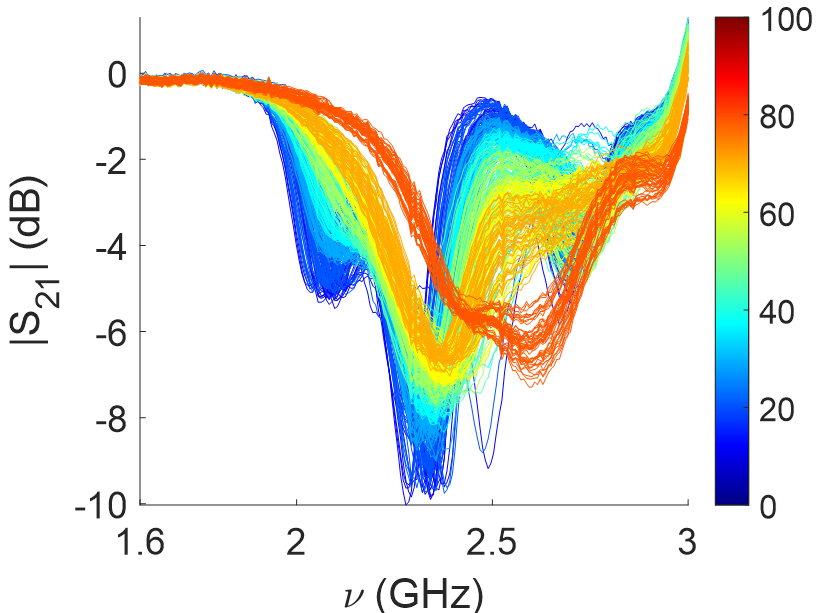
\includegraphics [trim = 0mm 0mm 0mm 0mm, clip, width=1\columnwidth]{figures/fig4_3.png}
	\caption{$20\dot{\log\left(|S_{21}|\right)}$ of each measurement contained in the generated dataset. Sampled concentrations of Ethanol in clean water ranges from $0\%$ and $96\%$. $10$ random commercial vials for each concentration were taken from a pool of $100$. $5$ rounds of measurements were performed. Each round consisted on measuring the $20\dot{\log\left(|S_{21}|\right)}$ of the CSRR when a random vial is picked and placed on top of the sensor, continuing and pass through the $90$ vials. Before each round, the $20\dot{\log\left(|S_{21}|\right)}$ of the CSRR unloaded was recorded for baseline correction of the data.}
	\label{fig:mlMeasTaken}
	\vspace{-0.3cm}
\end{figure}

\subsection{Principal Component Analysis}
\label{ssec:pcaAnalysis}

The many features shown by the generated dataset (see figure~\ref{fig:mlMeasTaken}) suggest that an exploratory analysis of the measurements is necessary. For this purpose, a Principal Component Analysis (PCA) was performed. In this analysis, the dataset was prepared and pre-processed as depicted in figure~\ref{fig:workflow} and the PCA was performed using the Statistics and Machine Learning Toolbox from MATLAB.

\begin{figure}[!t]
	\centering
	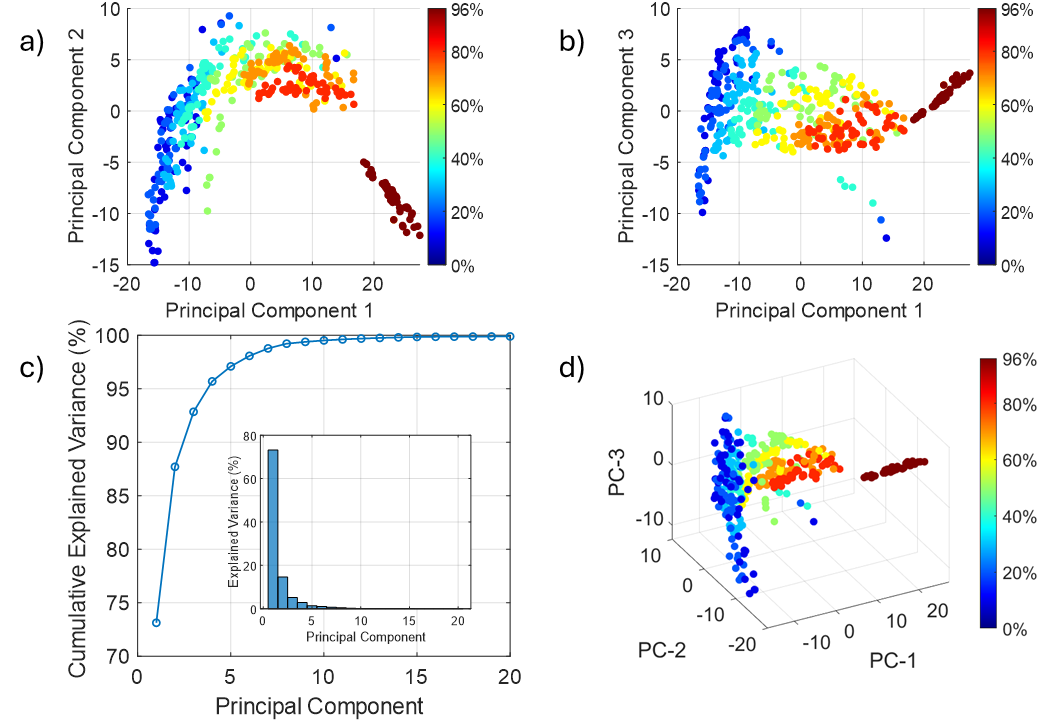
\includegraphics [trim = 0mm 0mm 0mm 0mm, clip, width=1\columnwidth]{figures/fig5_2.png}
	\caption{Principal Component Analysis (PCA) of the dataset generated as described in section~\ref{sssec:samplingML}. a) Distribution of each repetition in the reduced vectorial space when representing the second Principal Component (PC) with respect to the first PC. b) Distribution of each repetition in the reduced vectorial space when representing the third Principal Component (PC) with respect to the first PC. c) Cumulative Explained Variance of the dataset (in $\%$) with respect to the considered PCs and Explained Variance distribution over the set of PCs considered. d) 3D distribution of each repetition in the reduced vectorial space.}
	\label{fig:pcaAnalysis}
	\vspace{-0.3cm}
\end{figure}

As it is shown in figure~\ref{fig:workflow}, the dataset is cleaned by extracting the metadata (labels, date of acquisition, etc.) of the database and adjusting the number of features of each repetition if necessary. Then, the data matrix ($450\times201$) is pre-processed in two steps. First, each round of measurements is corrected in its baseline by using the $20\dot{\log\left(|S_{21}|\right)}$ of the unloaded CSRR. Second, each $20\dot{\log\left(|S_{21}|\right)}$ is auto-scaled by calculating the average, $\mu_{C}$, and de standard deviation, $\sigma_{C}$, for each concentration at each round.

As shown by figure~\ref{fig:pcaAnalysis}~(c), the $95\%$ of the Explained Variance (EV) is contained in the first four Principal Components (PCs). Most of this variance is accumulated in the first PC ($73\%$), and the rest show an EV lower than $15\%$. In particular, the fourth PC shows an EV lower than $3\%$.

Figures~\ref{fig:pcaAnalysis}~(a) and (b), show the distribution of the repetitions in the reduced vectorial space of the extracted PCs. In both figures, the first PC shows its dominance which can be related with the ethanol concentration in solution. The spread in this component shows that, despite the careful preparation of each stock solution, the system is sensitive enough to observe relatively small variations in concentration. 

Also, these figures show a spread in the second and third components which can be related to the variability introduced by the commercial vial and the actual measurement action (see figure~\ref{fig:pcaAnalysis}~(d)). Is in this variability where the outliers are observed. In particular, plot in figure~\ref{fig:pcaAnalysis}~(b) leads identify the outliers in concentrations of $0\%$, $20\%$ and $40\%$ shown in figure~\ref{fig:mlMeasTaken} and explained in section~\ref{sssec:samplingML}. 

The PCA analysis summarized in figure~\ref{fig:pcaAnalysis} might lead to chose one quantification ML algorithm from the variety of possibilities. In this case, as the EV concentrates in on PC, and for shake of simplicity, a linear predictor seams to be the most adequate choice.      

\subsection{Partial Least Squares Regressor}
\label{ssec:plsRegressor}

The PCA analysis presented in section~\ref{ssec:pcaAnalysis} suggests that a linear predictor of the concentration might be a good model for inference using the measurement of the $S_{21}$ parameter of a CSRR sensor embedded in the system presented in section~\ref{ssec:sysBlockD}. The most extended predictor is the Partial Least Squares Regressor (PLSR), especially suitable for datasets with short number of repetitions per sample~\cite{Wold2001}.

Figure~\ref{fig:workflow} shows the workflow developed for training and test of the PLSR. Once the database is acquired, in the Data Preparation step, the data is separated form metadata and adjusted to fit in a usable matrix. Also in this step, the baseline data ($20\dot{\log\left(|S_{21}|\right)}$ of the CSRR when unloaded) is separated from the database. These step results in a $450\times201$ feature matrix.

Before starting the PLSR training, the feature matrix was pre-processed. After a baseline correction of each set of $201$ features, the auto-scaling process was applied as explained in section~\ref{ssec:pcaAnalysis} so the resulting pre-processed feature matrix is the same as the used in the PCA study.   

The pre-processed data is then split in two different subsets. The data belonging to $6$ concentrations is used for training (training dataset) and the rest is left aside for final testing (test dataset). Therefore, the training dataset consisted in a $300\times201$ feature matrix and the test dataset in a $150\times201$. 

A double leave-one-block-out cross-validation (LOGO-CV) scheme is used for model training~\cite{Filzmoser2009}. This approach uses data from 4 rounds for model training and reserves one round for validation, resulting in 5 evaluations of different PLSR models. The model with best performance, in terms of Root Mean Square Error, is then selected. The LOGO-CV scheme is run for different number of Latent Variables up to 31. 

Once the PLSR model is trained, its evaluation is performed by introducing the test dataset and making predictions of the concentrations. In this case, predictions for $40\%$, $60\%$ and $80\%$ concentrations were calculated with the resulting model. These concentrations were chosen intentionally for compensating the presence of outliers (in $40\%$ for example) without having into account the both ends of the considered range of concentrations.

\begin{figure}[!t]
	\centering
	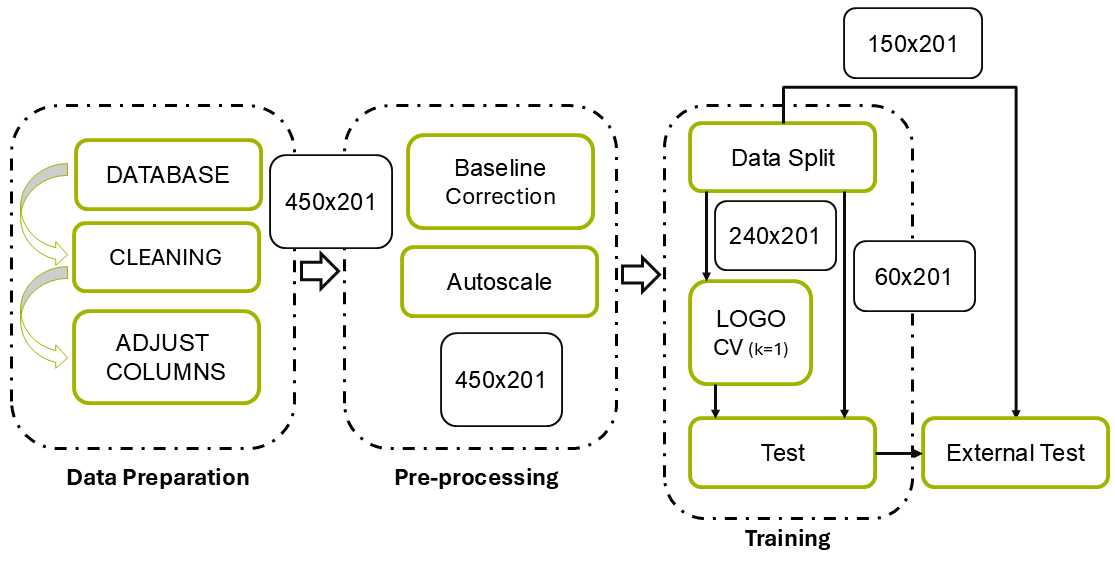
\includegraphics [trim = 0mm 0mm 0mm 0mm, clip, width=1\columnwidth]{figures/fig6_2.png}
	\caption{Block diagram of the developed workflow for training the bench-top CSRR system. In Data Preparation step, the database is cleaned by extracting the actual data (features) from metadata, providing a $450\times201$ feature matrix plus a $5\times201$ baseline matrix. In the Pre-Processing step the feature matrix baseline is correcte using the baseline matrix applied to each of the rounds separately. In the Training step, the feature matrix is split into the train dataset ($300\times201$ matrix) and the test dataset ($150\times201$ matrix). Then the train dataset is introduced in a leave-one-block-out cross-validation (LOGO-CV) training scheme which produces and optimized PLSR model. In the External Test step, the performance of the optimized model is evaluated by obtaining predictions from the test dataset.}
	\label{fig:workflow}
	\vspace{-0.3cm}
\end{figure}

Figure~\ref{fig:plsrStatistics}~(a) shows the evolution of the minimum Mean Square Error (MSE) with the number of components of the PLSR considered during the LOGO-CV scheme iteration. It is observed that with $6$ Latent Variables (LVs), the MSE of the best of the 5 models coming out from the LOGO-CV scheme is minimized up to $\sim6.8$ which leads to a Root Mean Square Error in Cross Validation (RMSECV) of $\sim3.62$. This values is very close to the error reported for the fitting presented in section~\ref{ssec:mlMeasurement} but here the time of sampling has been reduced to $\nicefrac{1}{4}$.

Also, the most important features in the training dataset were observed by using the Variable Importance in Projection (VIP) scores per each of the features~\cite{Chong2005}. The calculated scores provide information of the averaged importance of each feature in the projection of the repetition in the restricted vectorial space that handles the PLSR. This information can be used to trim the feature matrix columns to the most relevant part of the $20\dot{\log\left(|S_{21}|\right)}$.

There are many ways of defining the threshold that delimits which feature is more important than the rest~\cite{bibid}. However, a good first approach is to consider that every VIP score higher than $1$ belongs to a relevant feature. 

Figure~\ref{fig:plsrStatistics}~(b) shows the VIP scores for the training dataset once the PLSR is optimized to $6$ LVs. In this figure, pink areas (\squarecolor[pink]) show scores $>1$. It is observed that most important parts of the $20\dot{\log\left(|S_{21}|\right)}$ correspond to data close to $2.1$~GHz, $2.45$~GHz and $2.5$~GHz. These frequency spans correspond to the most relevant differences between concentrations observed in figure~\ref{fig:mlMeasTaken}.
 
\begin{figure}[!t]
	\centering
	\subfigure{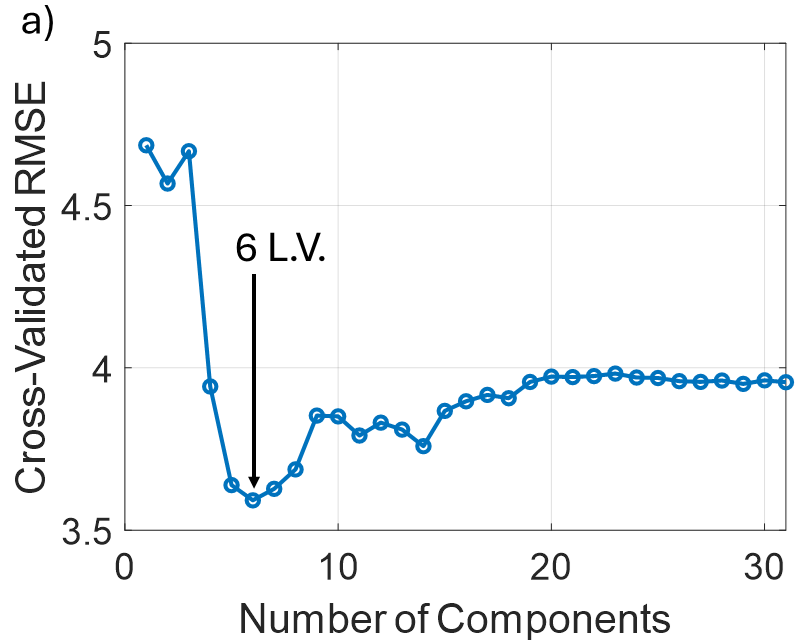
\includegraphics [trim = 0mm 0mm 0mm 0mm, clip, width=1\columnwidth]{figures/fig7_a.png}}
	\subfigure{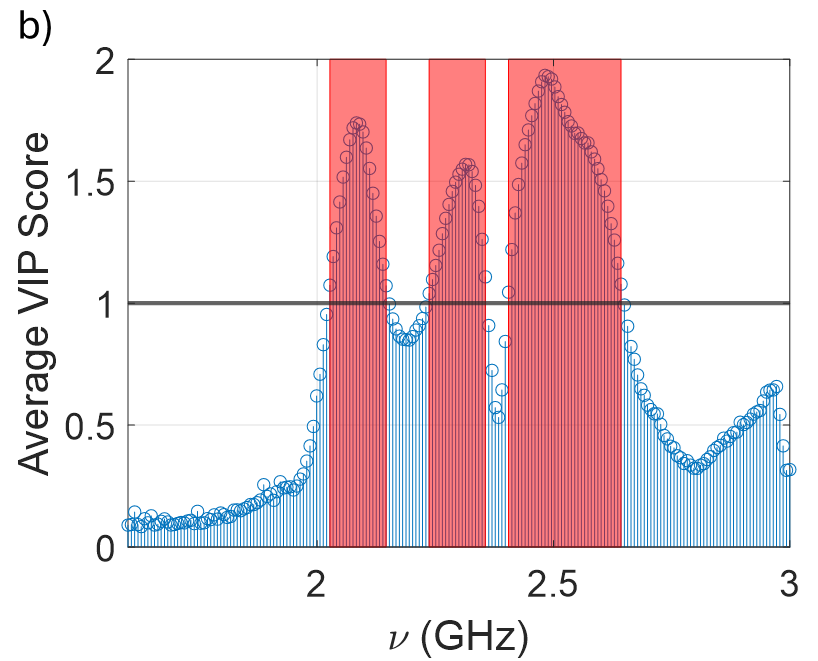
\includegraphics [trim = 0mm 0mm 0mm 0mm, clip, width=1\columnwidth]{figures/fig7_b.png}}
	%\hfill
	\caption{Statistics of the Partial Least Squares Regressor (PLSR) trained with the generated training dataset. a) Evolution of the Mean Square Error (MSE) with the number of Latent Variables (LV) during the Leave-One-Block-Out Cross Validation (LOGO-CV) training scheme. b) Mean Variable Importance in Projection (VIP) scores for each feature from $1.6$~GHz to $3$~GHz. The scores higher than 1 have been highlighted with \squarecolor[pink].}
	\label{fig:plsrStatistics}
\end{figure}

\section{CSRR System Performance}
\label{sec:csrrPerformance}
\subsection{Performance in Cross Validation}
\label{ssec:perfCV}

\begin{figure}[!t]
	\centering
	\subfigure{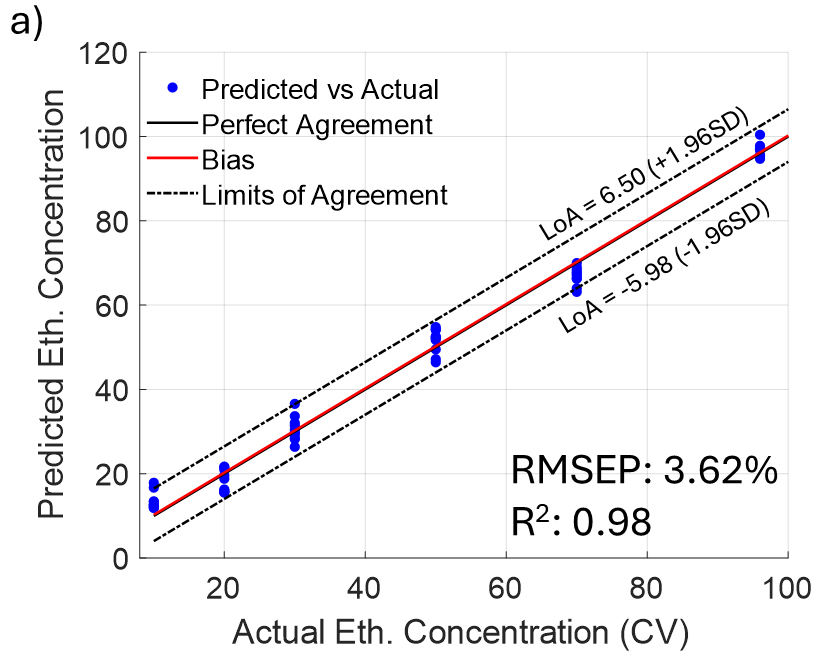
\includegraphics [trim = 0mm 0mm 0mm 0mm, clip, width=1\columnwidth]{figures/fig8_a.png}}
	\subfigure{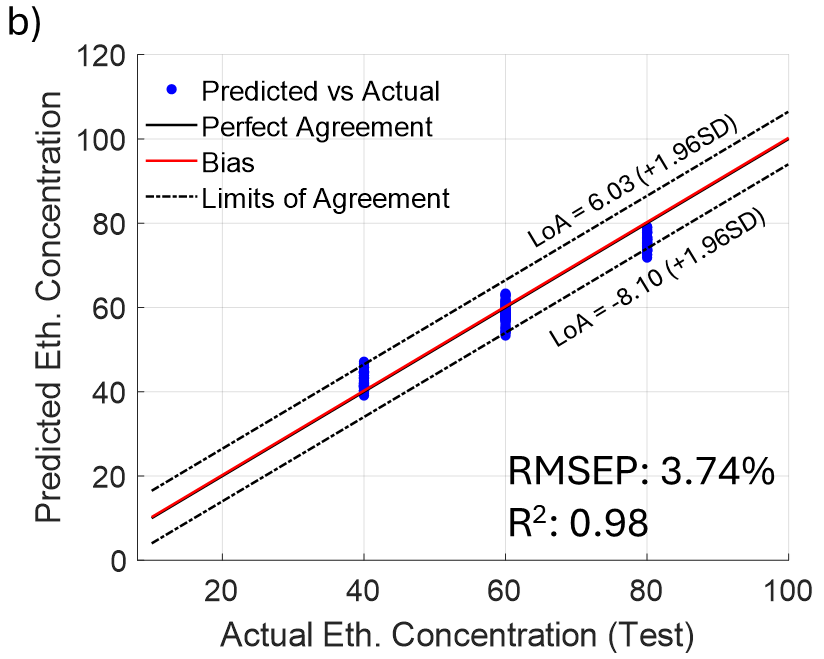
\includegraphics [trim = 0mm 0mm 0mm 0mm, clip, width=1\columnwidth]{figures/fig8_b.png}}
	%\hfill
	\caption{Statistics of the Partial Least Squares Regressor (PLSR) trained with the generated training dataset. a) Evolution of the Mean Square Error (MSE) with the number of Latent Variables (LV) during the Leave-One-Block-Out Cross Validation (LOGO-CV) training scheme. b) Mean Variable Importance in Projection (VIP) scores for each feature from $1.6$~GHz to $3$~GHz. The scores higher than 1 have been highlighted with \squarecolor[pink].}
	\label{fig:plsrResults}
\end{figure}

As mentioned in section~\ref{ssec:plsRegressor}, the LOGO-CV training scheme produces $5$ PLSR models per LVs considered during the training. From these $5$ models, the one with lower Root Mean Square Error (RMSE) is selected as representative of the LV set considered.

According with figure~\ref{fig:plsrStatistics}~(a), the PLSR model with $6$ LVs provides better performance during the LOGO-CV scheme. Therefore, this model was used to produce predictions on the training dataset. In this process, repetitions for $20\%$, $30\%$, $50\%$, $70\%$ and $96\%$ samples were part of the training dataset and the $20\%$ of these repetitions were kept aside for performance evaluation.

Figure~\ref{fig:plsrResults}~(a) shows the predictions of the PLSR model for the repetitions of the training dataset kept aside. The RMSE in CV (RMSECV) got close to $3.6$ with R$^{2}$ coefficient of $0.98$. The Limits of Agreement (LoA) were calculated using Blant-Altmand method for the $95\%$ of Confident Interval resulting in $13.5\%$ deviation from linear prediction.
 
\subsection{Performance in Test}
\label{ssec:perfTest}

Despite the test during training is performed with repetitions that the LOGO-CV scheme had no access to, it is interesting to test if the PLSR model is able to predict concentrations that the training process have not seen before. 

In section~\ref{ssec:plsRegressor}, the database was divided into training dataset and test dataset. The test dataset contained the repetitions of $40\%$, $60\%$ and $80\%$ samples. This dataset was used to obtain predictions with the PLSR model and evaluate its performance against "blind" samples.

Figure~\ref{fig:plsrResults}~(b) shows the predictions obtained for the test dataset. These predictions produced a RMSE in Prediction (RMSEP) about $3.7$, very close to the RMSECV, with a R$^{2}$ coefficient of $0.98$. The LoAs were calculated in the same way presented in previous section, resulting in a LoA~$\sim14.2\%$ with a $95\%$ of Confident Interval. 

The PLSR models showed a $1.5\%$ bias when predicting the concentrations of the test dataset and the LoAs increased also $\sim1\%$ with respect to the LoAs obtained in training. 

These performance was a bit worse than the performance shown during training but expected. The model has never put in contact with the data in the test dataset, therefore its variability might be different than the represented by the training dataset. However, the PLSR model trained following the scheme presented in section~\ref{ssec:plsRegressor} shows a good robustness against new repetitions of unknown samples.  

\section{Conclusions}
\label{sec:conclusion}

In this contribution, the impact of using Machine Learning Algorithms when measuring liquids with a CSRR based bench-top system is demonstrated. If properly applied, ML algorithms not only show the properties of the generated databases, but enhance the performance of systems predicting concentrations of SUTs in samples.

For a bench-top system like the presented in section~\ref{sec:csrrbenchTop}, the measurement procedure and the commercial vials used regularly in laboratories, introduce a considerable variability across repetitions. In the literature, this variability is managed, either enhancing the hardware of the system, which might be impossible in many of the cases, or by repeating measurements over samples. 

However, it has been demonstrated in section~\ref{sssec:sysCharac} that repeating measurements of samples, even considering different vials, results in datasets with large standard deviations and it is expected that a simple curve fitting will fail in predicting the concentration of the SUT. In particular, the presented system, measurement procedure and commercial vials resulted in standard deviations in dataset ranging from $8\%$ to $23\%$. These results make impossible to use this type of system in biomedical applications, where better accuracy is required.

As demonstrated in section~\ref{sec:csrrPerformance}, the application of ML techniques and algorithms might mitigate the observed lack of accuracy. Furthermore, an oriented sampling, that provides useful datasets (see section~\ref{ssec:mlMeasurement}), and a previous exploration of the obtained datasets, as explained in section~\ref{ssec:pcaAnalysis}, lead to a better understanding of the behaviour of CSRR bench-top systems. It also orientate to the proper prediction model useful for the application and the final use.

In particular, for the benchmark problem of ethanol concentration diluted in clean water, a PLS Regressor is the best choice, as argued in sections~\ref{ssec:pcaAnalysis} and~\ref{ssec:plsRegressor}. In fact, the trained model for this purpose shown a performance better than the curve fitting over a single characteristic of the response of the CSRR sensor with the SUT tipicaly presented in the literature. As shown in section~\ref{sec:csrrPerformance}, not only the RMSE is better over "blind" samples compared with curve fitting, but the LoAs are stable over samples and the prediction is robust all over the range of considered concentrations.    

It has been shown that the application of ML techniques and algorithms boost the performance of a CSRR based bench-top system. As a first serious approach to this topic, the contributions sets the procedures and the workflow that can open the door of biomedical applications to these type of measurement devices.

\section*{Acknowledgment}

Author want to thank Professor Antonio Pardo and Gema Guedes, Ph.D. for their collaboration during experiments in the laboratory and their understanding on the increasing entropy inside it.\\
Hola que tabular

\bibliographystyle{IEEEtran}
\bibliography{bib/ieeeBibCSRRandML}
%\vspace{-1cm}
\vskip -2\baselineskip plus -1fil

\begin{IEEEbiography}[{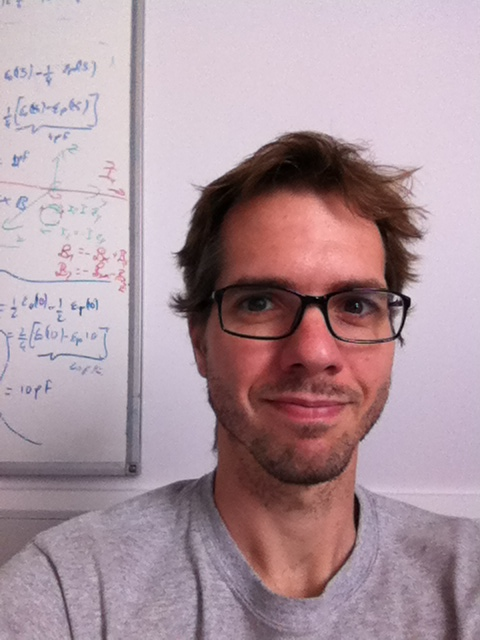
\includegraphics[width=1in,height=1.25in,clip,keepaspectratio]{figures/JAV-Website-Photo.jpg}}]{Javier Alonso-Valdesueiro}
was born in Madrid, Spain, in 1980. He earned a Telecommunications Engineering degree from the University of Alcalá, Madrid, in 2006, and a Ph.D. from the Polytechnic University of Catalonia, Barcelona, in 2011. From 2012 to 2020, he worked on developing electronic instrumentation for NMR experiments, initially at the C.E.A Center in France, followed by the University of Southampton in the UK, and later as a Marie Skłodowska-Curie Fellow at the University of the Basque Country (UPV/EHU). Over the past four years, he has advanced his career as an RF and instrumentation engineer in both private companies and public research centers, including TECNALIA Innovation Foundation and the Institute of Biomedical Engineering of Catalonia. Recently, he was appointed Assistant Professor in the Department of Electronic and Biomedical Engineering at the University of Barcelona. His current research focuses on radio-frequency (RF) devices for MRI, instrumentation electronics for gas sensing applications, and advancements in RF sensor technologies.
\end{IEEEbiography}
\vskip -2\baselineskip plus -1fil
%\vspace{-1.5cm}
\end{document}
